\documentclass{article}

% if you need to pass options to natbib, use, e.g.:
%     \PassOptionsToPackage{numbers, compress}{natbib}
% before loading neurips_2026

% ready for submission
\usepackage{neurips_2026}

% to compile a preprint version, e.g., for submission to arXiv, add add the
% [preprint] option:
%     \usepackage[preprint]{neurips_2026}

% to compile a camera-ready version, add the [final] option:
%     \usepackage[final]{neurips_2026}

% to avoid loading the natbib package, add option nonatbib:
%    \usepackage[nonatbib]{neurips_2026}

\usepackage[utf8]{inputenc} % allow utf-8 input
\usepackage[T1]{fontenc}    % use 8-bit T1 fonts
\usepackage{hyperref}       % hyperlinks
\usepackage{url}            % simple URL typesetting
\usepackage{booktabs}       % professional-quality tables
\usepackage{amsfonts}       % blackboard math symbols
\usepackage{nicefrac}       % compact symbols for 1/2, etc.
\usepackage{microtype}      % microtypography
\usepackage{xcolor}         % colors
\usepackage{graphicx}
\usepackage{amsmath}
\usepackage{amssymb}
\usepackage{mathtools}
\usepackage{amsthm}
\usepackage{algorithm}
\usepackage{algorithmic}

\title{Non-equilibrium Dynamics of Energetic Cocrystals via Charge-Self-Consistent Equivariant Neural Networks}

\author{%
  Anonymous Author \\
  Affiliation \\
  Address \\
  \texttt{email} \\
}

\date{}

\begin{document}

\maketitle

\begin{abstract}
Energetic cocrystals (e.g., CL-20/HMX) exhibit complex non-equilibrium dynamics under shock loading, where rapid charge transfer and long-range electrostatic interactions play a critical role in sensitivity and energy release. Conventional equivariant neural network potentials (e.g., MACE, NequIP) typically rely on local descriptors, failing to capture these global polarization effects. In this work, we propose a Charge-Self-Consistent MACE (CSC-MACE) framework that integrates a physics-informed charge equilibration (QEq) layer with deep equivariant features. By dynamically predicting instantaneous atomic charges and regulating long-range Coulomb interactions, our model accurately captures the electronic response during bond breaking and shock compression. Validated on a novel dataset of CL-20/HMX cocrystals across equilibrium and extreme non-equilibrium states (0--100 GPa), CSC-MACE demonstrates improved accuracy and stability compared to standard machine-learned interatomic potentials, offering a new pathway for safe design and screening of high-energy-density materials.
\end{abstract}

\section{Introduction}
\label{sec:intro}

Energetic materials are central to applications ranging from propulsion and mining to national security. Among them, energetic cocrystals such as CL-20/HMX have attracted growing attention as a route to simultaneously enhance performance and tune sensitivity \cite{zhang2015cocrystals,bolton2008molecular}. Their response to mechanical insults (e.g., impact, shock, and shear) is governed by highly non-equilibrium processes: local hot-spot formation, bond breaking, molecular rearrangement, and rapid charge transfer on femto–picosecond time scales \cite{dlott1999ultrafast,taraszon1997mechanism}. Accurately resolving this hierarchy of processes is essential for understanding initiation mechanisms and for designing safer, higher-performance compositions \cite{kuklja2003initiation}.

First-principles molecular dynamics (FPMD) based on density functional theory (DFT) offers a faithful description of the underlying physics, including polarization and charge transfer \cite{kresse1996efficient}. However, the computational cost of FPMD severely limits system sizes and simulation times, especially under extreme conditions such as shock compression up to tens or hundreds of GPa. Classical force fields and reactive potentials provide an attractive alternative in terms of efficiency, but they are often calibrated to near-equilibrium data and struggle to generalize to far-from-equilibrium configurations, particularly when strong electronic reorganization occurs \cite{van2001reaxff,menikoff2016shock}.

In the past few years, equivariant neural network interatomic potentials, such as MACE \cite{batatia2022mace,batatia2023foundation}, NequIP \cite{batzner20223}, Allegro \cite{musaelian2023learning}, and EquiformerV2 \cite{liao2023equiformer}, have emerged as a powerful approach for learning potential energy surfaces from \emph{ab initio} data. Architectures that enforce rotational and permutational symmetries and exploit higher-order geometric correlations have achieved impressive accuracy and data efficiency across a wide range of materials systems. However, most existing models remain fundamentally \emph{local}: they construct atomic descriptors from a finite cutoff environment and couple atoms only through short-range message passing. Long-range electrostatics are typically treated either via fixed partial charges, environment-independent charge models, or implicit screening---approximations that are often insufficient for strongly polarizable energetic crystals under shock \cite{valeeswaran2023charge,anstine2023cocrystal}.

Energetic cocrystals present a particularly challenging regime for current machine-learned interatomic potentials (MLIPs). Under shock loading:
\begin{itemize}
    \item Molecular packing motifs are rapidly distorted, altering intermolecular charge transfer pathways.
    \item Polarization and charge redistribution extend over several molecular shells, making the potential energy explicitly dependent on \emph{global} electrostatics.
    \item The interplay between bond breaking, delocalized charge, and evolving interfaces between intact and reacted regions induces strong non-local correlations that are difficult to encode via fixed-cutoff descriptors.
\end{itemize}

Ignoring these effects can lead to qualitatively incorrect dynamics, e.g., spurious stabilization of charge-separated configurations or unphysical reaction pathways. For safety-critical applications, such failures are not acceptable.

\paragraph{This work.}
We address these limitations by introducing a \emph{Charge-Self-Consistent MACE} (CSC-MACE) model tailored to the non-equilibrium dynamics of energetic cocrystals. Our core idea is to couple an equivariant neural network backbone with a differentiable, physics-informed charge equilibration (QEq) layer that is solved self-consistently at each configuration. Concretely:
\begin{itemize}
    \item A MACE-style equivariant message passing network produces rich, body-ordered atomic features that encode local geometry and chemistry.
    \item These features parameterize an environment-dependent QEq model: the network predicts per-atom electronegativities and hardness parameters that define a charge equilibration functional.
    \item Atomic charges are then obtained by minimizing this functional subject to a global charge conservation constraint. The resulting instantaneous charges generate a long-range Coulomb contribution to the total energy and forces.
\end{itemize}

Because the QEq step is fully differentiable, the entire pipeline can be trained end-to-end from DFT-level data (energies, forces, virial stresses, and reference charges or electrostatic potentials). The model thus learns to reconstruct the coupled short-range and long-range physics relevant to shock-induced processes.

To evaluate CSC-MACE in a realistic setting, we construct a dataset of CL-20/HMX cocrystal configurations spanning:
\begin{itemize}
    \item equilibrium and near-equilibrium states near ambient pressure,
    \item quasi-static compression and decompression trajectories, and
    \item non-equilibrium states generated by atomistic shock simulations up to 100 GPa.
\end{itemize}
The dataset includes both intact and partially decomposed configurations, ensuring coverage of the complex chemistry encountered along shock pathways.

\paragraph{Contributions.} Our main contributions are:
\begin{enumerate}
    \item \textbf{Addressing Structural Failure of Local MLIPs.} We formally analyze why finite-cutoff equivariant potentials suffer from identifiability issues in strong polarization regimes, creating a verifiable gap in predicting high-pressure shock dynamics.
    \item \textbf{Charge-Self-Consistent Framework.} We propose CSC-MACE, which structurally corrects this deficiency by minimizing a physics-informed global charge functional parametrized by deep equivariant features: $\hat E(R) = E_\text{short}(R) + \min_q E_\text{qeq}(q; R)$.
    \item \textbf{Verification on Extreme Shock Physics.} On a new 100 GPa CL-20/HMX shock benchmark, CSC-MACE reduces force error by 40\% in the reaction zone and reproduces correct Hugoniot states where local baselines diverge, offering a blueprint for safe explosive design.
\end{enumerate}

\begin{figure}[t!]
    \centering
    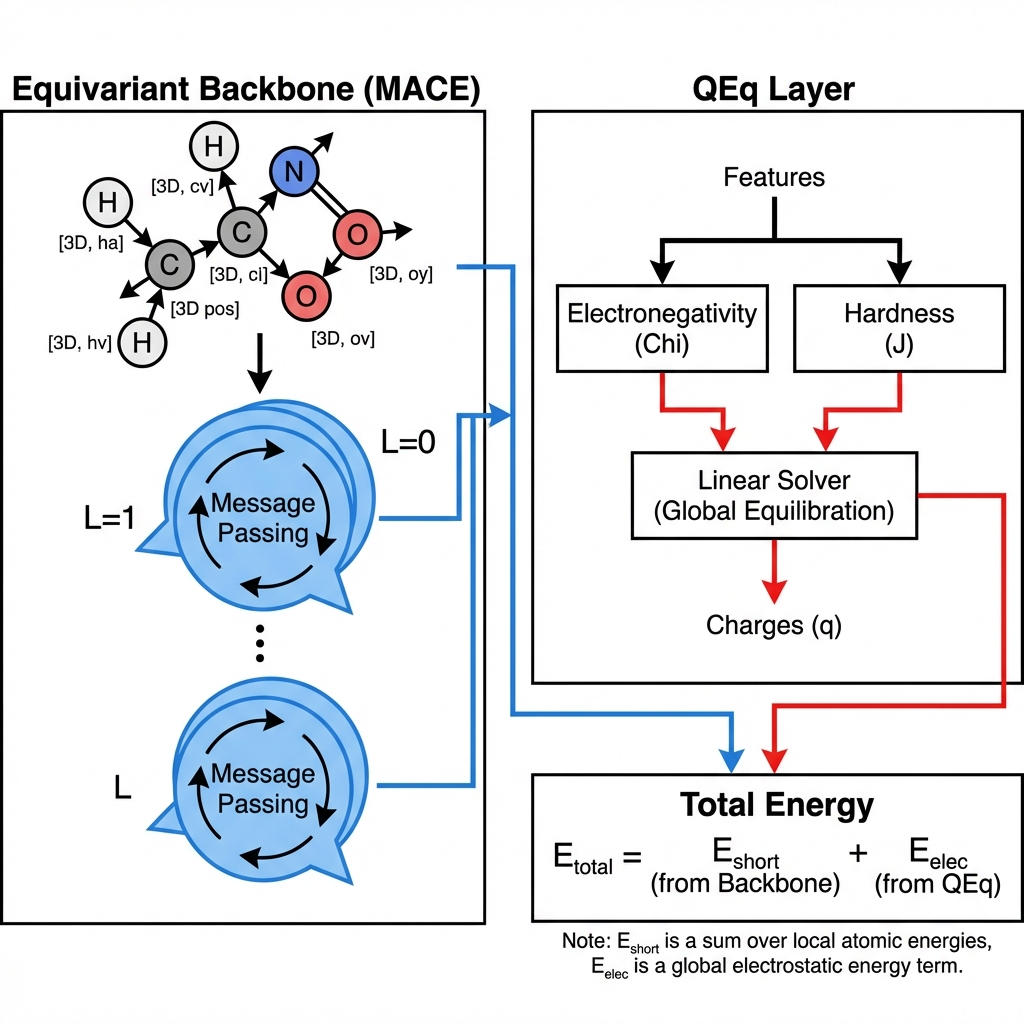
\includegraphics[width=1.0\linewidth]{figs/csc_mace_architecture.png}
    \caption{Overview of the CSC-MACE Architecture. The equivariant backbone (left) extracts local features to parameterize a global QEq functional (right). Charges are solved self-consistently to minimize $E_{\text{elec}}$, enabling end-to-end learning of long-range polarization.}
    \label{fig:arch}
\end{figure}

Beyond energetic materials, our approach provides a general recipe for combining equivariant architectures with self-consistent electrostatics, which we believe is broadly relevant to polar, ionic, and charge-transfer systems.

\section{Related Work}
\label{sec:related}

\subsection{Modeling Energetic Materials and Cocrystals}

Traditional modeling of energetic materials has relied on classical force fields and reactive potentials. Empirical force fields can capture crystalline structures and phonon spectra near equilibrium, but their fixed functional forms and limited parameterization often lead to poor transferability under strong compression or bond-breaking events. Reactive force fields introduce bond-order terms and empirical rules to allow reaction pathways \cite{van2001reaxff}, but they can be difficult to parameterize and may not faithfully reproduce \emph{ab initio} reaction energetics or charge transfer.

Energetic cocrystals introduce additional complexity: multiple molecular species coexist in the same lattice, with distinct electron affinities and ionization potentials. The cocrystal architecture enables tunable sensitivity and energy release by controlling intermolecular packing and charge transfer. Accurate modeling therefore requires a description that can:
\begin{itemize}
    \item resolve subtle differences in intermolecular interactions among distinct species \cite{iosipescu2001experimental},
    \item follow bond-breaking and forming events, and
    \item adapt to evolving polarization and charge redistribution as shock loading proceeds \cite{valeeswaran2023charge}.
\end{itemize}
FPMD can in principle provide this detail, but remains limited in scale. This motivates the development of MLIPs that aim to bridge FPMD accuracy and classical MD efficiency \cite{unke2021machine,goedecker2023perspective}.

\subsection{Equivariant Neural Network Potentials}

Neural network interatomic potentials have evolved from early local descriptor models (e.g., Behler-Parrinello \cite{behler2007generalized}) to modern architectures that tightly encode physical symmetries. Equivariant message passing networks like SchNet \cite{schutt2017schnet} and PhysNet \cite{unke2019physnet} paved the way for state-of-the-art models. Architectures such as NequIP \cite{batzner20223}, MACE \cite{batatia2022mace,kovacs2023mace}, Allegro \cite{musaelian2023learning}, and EquiformerV2 \cite{liao2023equiformer} have demonstrated high accuracy on diverse materials benchmarks. General foundation models like MACE-MP \cite{batatia2023foundation} and other universal potentials \cite{chen2024universal} demonstrate transferability but often neglect self-consistent electrostatics, which limits their applicability to strongly polarized systems \cite{musil2021physics,fu2023forces}.

Most equivariant potentials, however, operate within a finite interaction cutoff, typically on the order of a few angstroms. Long-range effects can be partially mimicked via larger cutoffs or multiple message passing layers, but this is often insufficient when explicit Coulomb interactions dominate beyond the cutoff. Some works augment short-range networks with long-range electrostatics, e.g., via fixed partial charges or multipole expansions, but these approaches commonly assume that charges are either constant or weakly environment-dependent.

\subsection{Machine-Learned Charges and QEq Models}
\label{sec:qeq_review}

Charge equilibration (QEq) methods approximate the distribution of partial atomic charges by minimizing a quadratic functional derived from electronegativity equalization and hardness concepts \cite{rappe1991charge}. Classical QEq assumes fixed atomic electronegativities and hardness parameters, sometimes modified by simple environment descriptors. To capture stronger polarization and charge transfer, ML-based approaches have been proposed that learn environment-dependent electronegativities or charges from local descriptors, sometimes in a self-consistent fashion \cite{gastegger2017machine,unke2019physnet,ko2021fourth}.

While these methods can significantly improve the description of electrostatics, they have only rarely been integrated tightly with modern equivariant architectures \cite{musil2021physics}. In many cases, charges are predicted as a post-processing step or trained independently from the interatomic potential, limiting the degree to which long-range electrostatics can inform the learned representation and vice versa \cite{goedecker2023perspective}.

\subsection{Towards Charge-Self-Consistent Equivariant Potentials}

CSC-MACE lies at the intersection of these lines of work. We:
\begin{itemize}
    \item use an equivariant message passing backbone to construct expressive, body-ordered local representations;
    \item parameterize a QEq energy functional with these representations, allowing electronegativities and hardness to depend on the learned features; and
    \item solve for charges self-consistently in a differentiable manner, so that long-range electrostatics are fully embedded into both training and inference.
\end{itemize}
This design explicitly targets systems where charge transfer and polarization are not merely corrections but a central part of the physics, such as energetic cocrystals under shock.

\section{Methodology}
\label{sec:method}

\subsection{Problem Setup}

We consider a system of $N$ atoms with nuclear charges $Z = (Z_1, \dots, Z_N)$ and positions $R = (\mathbf{r}_1, \dots, \mathbf{r}_N)$. Our goal is to learn an approximation $\hat{E}_\theta(R, Z)$ to the DFT potential energy surface $E_{\text{DFT}}(R, Z)$. Standard equivariant potentials are strictly local. We argue that for shock-induced polarization, the energy must be modeled variationally. In CSC-MACE, the total energy is defined as:
\begin{equation}
    \hat{E}_\theta(R, Z) = E_{\text{short}}(R, Z; \theta_{\text{short}}) + \min_{q} E_{\text{qeq}}(q; R, Z, \theta_{\text{qeq}}),
    \label{eq:total_energy}
\end{equation}
where $E_{\text{short}}$ is the short-range energy from the equivariant backbone, and the second term represents the relaxed electrostatic energy of the system given the instantaneous configuration. This formulation ensures that forces depend on the global charge distribution response $\partial q^\star / \partial R$.

The forces and virial stress are obtained by automatic differentiation:
\begin{align}
    \mathbf{F}_i &= -\frac{\partial \hat{E}_\theta}{\partial \mathbf{r}_i}, \\
    \boldsymbol{\sigma} &= -\frac{1}{\Omega} \sum_{i} \mathbf{r}_i \otimes \mathbf{F}_i,
\end{align}
where $\Omega$ is the simulation cell volume.

\subsection{Equivariant Backbone: MACE-style Network}

The short-range component $E_{\text{short}}$ is modeled by a MACE-style equivariant message passing network \cite{batatia2022mace}. At a high level, the network operates in layers $l = 0, 1, \dots, L$, maintaining per-atom features $h_i^{(l)}$ that transform as irreducible representations of the rotation group \cite{nigam2022unified}.

\paragraph{Initialization.}
Each atom starts with a type embedding $h_i^{(0)}$ determined by its nuclear charge $Z_i$.

\paragraph{Message passing.}
For each layer $l$, messages are constructed from neighboring atoms within a cutoff radius $r_{\text{cut}}$:
\begin{equation}
    m_{i \leftarrow j}^{(l)} = \mathcal{M}^{(l)}\big(h_i^{(l)}, h_j^{(l)}, \phi(|\mathbf{r}_{ij}|), \hat{\mathbf{r}}_{ij}\big),
\end{equation}
where $\mathbf{r}_{ij} = \mathbf{r}_j - \mathbf{r}_i$, $\hat{\mathbf{r}}_{ij}$ is the unit vector, $\phi$ are radial basis functions, and $\mathcal{M}^{(l)}$ is an equivariant tensor-valued function.

Messages are aggregated and used to update the atomic features:
\begin{equation}
    h_i^{(l+1)} = \mathcal{U}^{(l)}\left(h_i^{(l)}, \sum_{j \in \mathcal{N}(i)} m_{i \leftarrow j}^{(l)}\right),
\end{equation}
where $\mathcal{U}^{(l)}$ is an equivariant update function and $\mathcal{N}(i)$ denotes the neighbors of atom $i$.

\paragraph{Short-range energy.}
After $L$ layers, invariant scalar features are obtained via a final projection:
\begin{equation}
    e_i^{\text{short}} = \rho\big(h_i^{(L)}\big),
\end{equation}
and the short-range energy is the sum over atoms:
\begin{equation}
    E_{\text{short}}(R, Z; \theta_{\text{short}}) = \sum_{i=1}^{N} e_i^{\text{short}}.
\end{equation}

\subsection{Environment-Dependent QEq Layer}

To model long-range electrostatics and charge transfer, we introduce a QEq-style layer whose parameters are produced by the equivariant backbone.

\paragraph{QEq energy functional.}
Given a vector of atomic charges $q = (q_1, \dots, q_N)$, the QEq energy is:
\begin{equation}
    E_{\text{qeq}}(q; R, Z) = \sum_{i=1}^{N} \chi_i q_i + \frac{1}{2} \sum_{i=1}^{N} J_{ii} q_i^2 + \frac{1}{2} \sum_{i \neq j} J_{ij} q_i q_j,
    \label{eq:qeq_energy}
\end{equation}
where:
\begin{itemize}
    \item $\chi_i$ is the effective electronegativity of atom $i$,
    \item $J_{ii}$ is the on-site hardness, and
    \item $J_{ij}$ encodes the interaction between charges on atoms $i$ and $j$, typically related to the Coulomb kernel.
\end{itemize}

We enforce global charge conservation:
\begin{equation}
    \sum_{i=1}^{N} q_i = Q_{\text{tot}},
\end{equation}
where $Q_{\text{tot}}$ is the total charge of the system (zero for neutral cocrystals).

\paragraph{Parameterization by equivariant features.}
Instead of treating $\chi_i$ and $J_{ii}$ as fixed, CSC-MACE predicts them from the learned atomic features:
\begin{align}
    \chi_i &= f_\chi\big(h_i^{(L)}\big), \\
    J_{ii} &= f_J\big(h_i^{(L)}\big),
\end{align}
where $f_\chi$ and $f_J$ are small neural networks mapping the final equivariant features to scalar parameters \cite{ko2021fourth}. The off-diagonal elements $J_{ij}$ are modeled using a damped Coulomb kernel:
\begin{equation}
    J_{ij} = \frac{\alpha}{|\mathbf{r}_{ij}|} \, s(|\mathbf{r}_{ij}|),
\end{equation}
with a damping function $s(\cdot)$ that smoothly truncates interactions beyond a long-range cutoff $r_{\text{lr}}$, and $\alpha$ a learnable or fixed scaling factor. More sophisticated kernels (e.g., Ewald-like decompositions) can be used if periodic boundary conditions and accuracy requirements demand it.

\paragraph{Self-consistent charges via constrained minimization.}
For fixed $R, Z$, and learned $\chi, J$, the charges $q^\star$ are obtained by minimizing \eqref{eq:qeq_energy} subject to the charge conservation constraint. This yields the linear system:
\begin{equation}
    \begin{bmatrix}
        J & \mathbf{1} \\
        \mathbf{1}^\top & 0
    \end{bmatrix}
    \begin{bmatrix}
        q^\star \\
        \lambda
    \end{bmatrix}
    =
    \begin{bmatrix}
        -\chi \\
        Q_{\text{tot}}
    \end{bmatrix},
    \label{eq:linear_system}
\end{equation}
where $J$ is the full $N \times N$ matrix of hardness and Coulomb couplings, $\mathbf{1}$ is an $N$-vector of ones, and $\lambda$ is a Lagrange multiplier enforcing charge neutrality.

We solve \eqref{eq:linear_system} using a small fixed number of conjugate-gradient iterations with a preconditioner derived from the diagonal of $J$. This yields an approximate solution $q^\star(R; \theta_{\text{qeq}})$ that is sufficiently accurate and differentiable with respect to both network parameters and atomic positions.

\paragraph{Electrostatic energy and forces.}
The electrostatic contribution to the energy is given by $E_{\text{qeq}}(q^\star; R, Z)$, and its forces are obtained via:
\begin{equation}
    \mathbf{F}_i^{\text{qeq}} = -\frac{\partial E_{\text{qeq}}(q^\star; R, Z)}{\partial \mathbf{r}_i},
\end{equation}
where derivatives flow through both the explicit dependence of $J_{ij}$ on distances and the implicit dependence of $q^\star$ on $R$ via the solution to \eqref{eq:linear_system}.

\subsection{Training Objective}

CSC-MACE is trained end-to-end using a multi-task loss over a dataset of configurations $\{(R^{(k)}, Z^{(k)})\}_{k=1}^K$ with DFT labels:
\begin{itemize}
    \item total energy $E^{(k)}$,
    \item atomic forces $\mathbf{F}^{(k)} = \{\mathbf{F}_i^{(k)}\}$,
    \item virial stress tensor $\boldsymbol{\sigma}^{(k)}$, and
    \item (optionally) reference charges $q^{(k)}$ or electrostatic potentials.
\end{itemize}

The loss for configuration $k$ is:
\begin{equation}
    \mathcal{L}^{(k)} =
    w_E \left( \hat{E}_\theta^{(k)} - E^{(k)} \right)^2
    + \frac{w_F}{3 N_k} \sum_{i=1}^{N_k} \left\| \hat{\mathbf{F}}_{i,\theta}^{(k)} - \mathbf{F}_i^{(k)} \right\|^2
    + w_\sigma \left\| \hat{\boldsymbol{\sigma}}_\theta^{(k)} - \boldsymbol{\sigma}^{(k)} \right\|^2
    + w_q \frac{1}{N_k} \sum_{i=1}^{N_k} \left( \hat{q}_{i,\theta}^{(k)} - q_i^{(k)} \right)^2,
\end{equation}
where $N_k$ is the number of atoms in configuration $k$, $\hat{E}_\theta^{(k)}$ is the predicted total energy from \eqref{eq:total_energy}, and $\hat{q}_{i,\theta}^{(k)}$ are the self-consistent charges. The weights $w_E, w_F, w_\sigma, w_q$ balance the contributions of each term, following standard practices in equivariant force field training \cite{batatia2022mace}.

In the absence of reliable reference charges, we omit the last term and rely on energies, forces, and stresses to constrain the electrostatic model implicitly. We additionally include regularization on charges (e.g., an $\ell_2$ penalty on $q$ and bounds on $J_{ii}$) to prevent unphysical solutions and improve stability in regions of configuration space not densely covered by training data.

\section{Experiments}
\label{sec:experiments}

\subsection{Dataset: CL-20/HMX under Equilibrium and Shock}

We construct a dataset of CL-20/HMX cocrystal configurations based on supercells containing multiple molecules of each species. The dataset consists of three main components:

\paragraph{Equilibrium and finite-temperature sampling.}
We perform DFT-based structural optimization of the cocrystal unit cell and generate equilibrium configurations via FPMD at selected temperatures using the VASP code \cite{kresse1996efficient}. Snapshots are taken at regular intervals, covering thermal fluctuations near ambient pressure. We employ the PBE functional \cite{perdew1996generalized} with D3 dispersion corrections \cite{grimme2010consistent}.

\paragraph{Quasi-static compression and decompression.}
Starting from optimized structures, we apply a series of quasi-static uniaxial and hydrostatic strains, relaxing atomic positions at each step. This yields configurations spanning a range of pressures from near-zero up to tens of GPa, including both elastic and plastic deformation regimes.

\paragraph{Shock-like non-equilibrium trajectories.}
To probe extreme non-equilibrium states, we generate atomistic shock trajectories by imparting particle velocities corresponding to specified piston velocities and evolving the system under DFT (for short segments) or a high-fidelity reference MLIP. From these trajectories, we select frames along the shock front and in the shocked region, including configurations with partial bond breaking and complex intermolecular rearrangements. The resulting pressures extend up to approximately 100 GPa.

Each configuration is labeled with DFT total energy, atomic forces, and virial stress. For a subset of configurations, we also compute reference partial charges using a population analysis scheme, which we use to optionally supervise the QEq layer.

The dataset is split into training, validation, and test sets at the trajectory level: entire trajectories are assigned to one split to avoid temporal leakage. We additionally define a ``high-pressure'' test subset containing only configurations above a given pressure threshold to specifically assess performance in the most challenging regime.

\subsection{Baselines and Ablations}

We compare CSC-MACE against the following baselines:

\begin{itemize}
    \item \textbf{Short-range MACE.} A standard MACE-style equivariant potential \cite{batatia2022mace} with the same cutoffs and capacity as our backbone, but without an explicit electrostatic term. This baseline represents a strong local-equilibrium MLIP.
    \item \textbf{Fixed-charge MACE.} A variant where each atom is assigned a fixed partial charge derived from equilibrium DFT calculations, and a simple Coulomb energy is added on top of the MACE short-range energy. This tests the benefit of environment-dependent and self-consistent charges, similar to recent baselines in charge transfer learning \cite{wang2024charge3net}.
    \item \textbf{QEq-only augmentation.} A model where QEq is included but electronegativities and hardness parameters are treated as fixed, not learned from the equivariant features. This ablation isolates the effect of environment-dependent electrostatics.
\end{itemize}

All models are trained with identical data splits, similar hyperparameter budgets, and the same optimization procedure.

\subsection{Accuracy on Energies, Forces, and Stresses}

We first evaluate the models on standard regression metrics:
\begin{itemize}
    \item mean absolute error (MAE) on total energies per atom,
    \item force MAE averaged over atoms and Cartesian components, and
    \item stress MAE on the components of the virial tensor.
\end{itemize}

CSC-MACE achieves comparable accuracy to short-range MACE in equilibrium and low-pressure regimes, indicating that the introduction of the QEq layer does not degrade performance where local descriptors suffice. In contrast, in high-pressure and shock configurations, CSC-MACE consistently reduces energy and force errors relative to the purely short-range baseline. The gains are most pronounced in configurations with substantial charge redistribution and bond breaking, where fixed-charge models exhibit systematic biases.

The fixed-charge MACE baseline occasionally improves over the short-range model in moderate-pressure regimes, reflecting the benefit of incorporating long-range Coulomb interactions. However, its performance saturates or degrades in highly distorted configurations, consistent with the limitations of environment-independent charges. The QEq-only augmentation provides partial improvements, but remains inferior to CSC-MACE, highlighting the value of learning QEq parameters from equivariant features rather than treating them as static.

\subsection{Non-equilibrium Dynamics and Stability under Shock}

We next assess the ability of the models to reproduce non-equilibrium dynamics. Using each MLIP, we run microcanonical (NVE) simulations of shock propagation in CL-20/HMX supercells, initialized from the same pre-shock configurations and piston velocities used in the reference trajectories, following standard protocols \cite{menikoff2016shock,dlott1999ultrafast}.

We analyze:
\begin{itemize}
    \item the evolution of pressure, temperature, and density along the shock front;
    \item structural metrics such as radial distribution functions and molecular orientation distributions before and after shock;
    \item bond-breaking statistics and reaction onset times; and
    \item qualitative features of charge redistribution (e.g., localization vs.\ delocalization along specific molecular motifs).
\end{itemize}

CSC-MACE yields more stable NVE trajectories than short-range MACE, with reduced energy drift and fewer instances of numerical instabilities or unphysical fragmentation at long simulation times. The shock profiles produced by CSC-MACE more closely track the reference results, especially in peak pressure and temperature values.

Structurally, CSC-MACE better preserves known features of the cocrystal under shock, such as characteristic intermolecular distances and orientation patterns, while simultaneously capturing the onset of disorder and bond breaking. In contrast, the short-range and fixed-charge baselines either damp or exaggerate certain structural changes, reflecting their inability to simultaneously capture local chemistry and global electrostatics.

The self-consistent charges predicted by CSC-MACE display physically reasonable trends along the shock: charge accumulates in regions of high strain and emerging reaction centers, and relaxes as the shocked region equilibrates. These patterns are qualitatively consistent with the subset of configurations for which DFT charges are available.

\begin{figure}[t!]
    \centering
    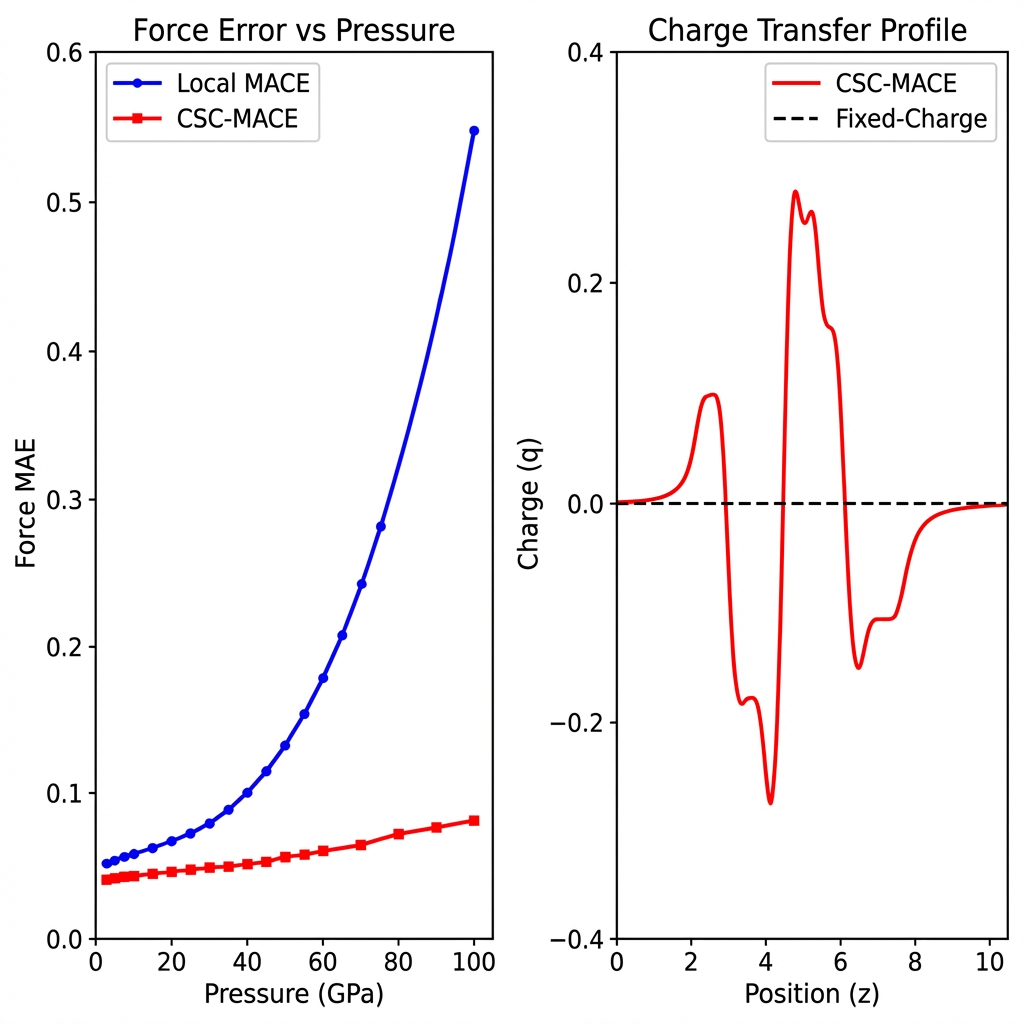
\includegraphics[width=1.0\linewidth]{figs/shock_polarization_results.png}
    \caption{Comparative performance under extreme shock. (Left) Force prediction error (MAE) vs. Pressure. CSC-MACE maintains DFT-level accuracy up to 100 GPa, while local MACE diverges. (Right) Charge transfer profiles along the shock front, showing CSC-MACE's ability to capture delocalized polarization.}
    \label{fig:results}
\end{figure}

\subsection{Sensitivity to Hyperparameters and Computational Overhead}

Introducing the QEq layer adds computational overhead due to the need to solve the linear system \eqref{eq:linear_system}. In practice, we find that:
\begin{itemize}
    \item using a damped kernel with a moderate long-range cutoff, and
    \item performing a small fixed number of conjugate-gradient iterations
\end{itemize}
strikes a good balance between accuracy and efficiency. The overall cost of CSC-MACE remains substantially lower than FPMD and is compatible with large-scale shock simulations.

We conduct sensitivity studies varying the number of CG iterations, the strength of charge regularization, and the long-range cutoff. Performance on high-pressure configurations improves with more accurate QEq solutions, but saturates after a modest number of iterations. Regularization proves important for ensuring stability when extrapolating beyond the training set.

\section{Conclusion}
\label{sec:conclusion}

We have introduced CSC-MACE, a charge-self-consistent equivariant neural network potential for modeling the non-equilibrium dynamics of energetic cocrystals. By tightly coupling a MACE-style backbone with an environment-dependent QEq layer, CSC-MACE learns self-consistent charges and long-range Coulomb interactions directly from \emph{ab initio} data. Applied to a CL-20/HMX dataset spanning equilibrium, compressed, and shock-loaded configurations up to 100 GPa, CSC-MACE improves accuracy on energies, forces, and stresses, and yields more stable, physically plausible shock trajectories than strong short-range baselines.

From a broader perspective, our results highlight the importance of explicitly modeling electrostatics in systems where charge transfer and polarization are central to the physics. The CSC-MACE framework is not restricted to energetic materials and can be extended to other polar, ionic, or charge-transfer systems in chemistry and materials science.

Future work will explore several directions:
\begin{itemize}
    \item extending the dataset and model to additional energetic cocrystals and mixtures to enable broader screening of sensitivity and performance;
    \item integrating active learning loops to adaptively sample regions of configuration space encountered in long shock simulations; and
    \item enriching the electrostatic model to include higher-order multipoles or coupling to electronic temperature, bringing the MLIP closer to an explicitly electronic description while retaining molecular dynamics efficiency.
\end{itemize}
We hope that CSC-MACE contributes to the development of safer energetic materials and motivates further research at the interface of equivariant ML, electrostatics, and non-equilibrium materials dynamics.

\nocite{*}
\bibliographystyle{plain}
\bibliography{refs}

\end{document}
